\section{Empennage}

\begin{tabularx}{\textwidth}{ | L | c | c | }
  \hline
  \textbf{Parameter}                    & \textbf{Value}   & \textbf{Reference} \\ \hline
  \endfirsthead
  \hline
  \textbf{Parameter}                    & \textbf{Value}   & \textbf{Reference} \\ \hline
  \endhead
  Horizontal tail span                  & 4.38 m           & \cite{NASA-CR-166309} \\ \hline
  Horizontal tail area                  & 4.18 m\textsuperscript{2} & \cite{Janes20042005,NASA-CR-166309} \\ \hline
  Horizontal tail root chord            & 1.12 m           & \cite{NASA-CR-166309} \\ \hline
  Horizontal tail tip chord             & 0.77 m           & \cite{NASA-CR-166309} \\ \hline
  Horizontal tail sweep (0.25MAC)       & 0.0\degree       & \cite{NASA-CR-166309} \\ \hline
  Horizontal tail aspect ratio          & 4.6              & \cite{NASA-CR-166309} \\ \hline
  Horizontal tail airfoil               & NACA 0014        & \cite{NASA-CR-166309} \\ \hline
  Horizontal tail stationline           & 17.79 m          & \cite{NASA-CR-166309,NASA-TM-85890} \\ \hline
  Horizontal tail waterline             & 6.20 m           & \cite{NASA-CR-166309,NASA-TM-85890} \\ \hline
  Horizontal tail deflection limit      & up -30\degree, down +35\degree & \cite{UH60_OperatorsManual} \\ \hline
  Vertical tail span                    & 2.49 m           & \cite{NASA-CR-166309} \\ \hline
  Vertical tail area                    & 3.00 m\textsuperscript{2} & \cite{Janes20042005,NASA-CR-166309} \\ \hline
  Vertical tail root chord              & 1.83 m           & \cite{NASA-CR-166309} \\ \hline
  Vertical tail tip chord               & 0.86 m           & \cite{NASA-CR-166309} \\ \hline
  Vertical tail sweep (0.25MAC)         & 41.0\degree      & \cite{NASA-CR-166309} \\ \hline
  Vertical tail aspect ratio            & 1.92             & \cite{NASA-CR-166309} \\ \hline
  Vertical tail airfoil                 & NACA 0021 (Mod)  & \cite{NASA-CR-166309} \\ \hline
  Vertical tail stationline             & 17.65 m          & \cite{NASA-CR-166309,NASA-TM-85890} \\ \hline
  Vertical tail waterline               & 6.93 m           & \cite{NASA-CR-166309,NASA-TM-85890} \\ \hline
  \caption{Empennage data}
\end{tabularx}

%%%%%%%%%%%%%%%%%%%%%%%%%%%%%%%%%%%%%%%%%%%%%%%%%%%%%%%%%%%%%%%%%%%%%%%%%%%%%%%%

\clearpage
\subsection{Main Rotor Inplane Wash at the Horizontal Tail}

\csvreader[
  no head,
  longtable=cccc,
  table head=
    \toprule
    $\chi$ & \multicolumn{3}{c}{EKXH1} \\
    {[deg]} & {AA1FMR=-6.0} & {AA1FMR=0.0} & {AA1FMR=6.0} \\ \midrule
    \endfirsthead
    $\chi$ & \multicolumn{3}{c}{EKXH1} \\
    {[deg]} & {AA1FMR=-6.0} & {AA1FMR=0.0} & {AA1FMR=6.0} \\ \midrule
    \endhead,
  before first line={},
  late after line=\\,
  late after last line=\\ \bottomrule \caption{Main rotor inplane wash at the horizontal tail \cite{NASA-CR-166309}},
  before reading={},
  after reading={}
]
{csv/uh60_stab_h_mr_inplane.csv}
{1=\colchi,2=\colii,3=\coliii,4=\coliv}
{\colchi & \colii & \coliii & \coliv}

\begin{figure}[h!]
  \centering
  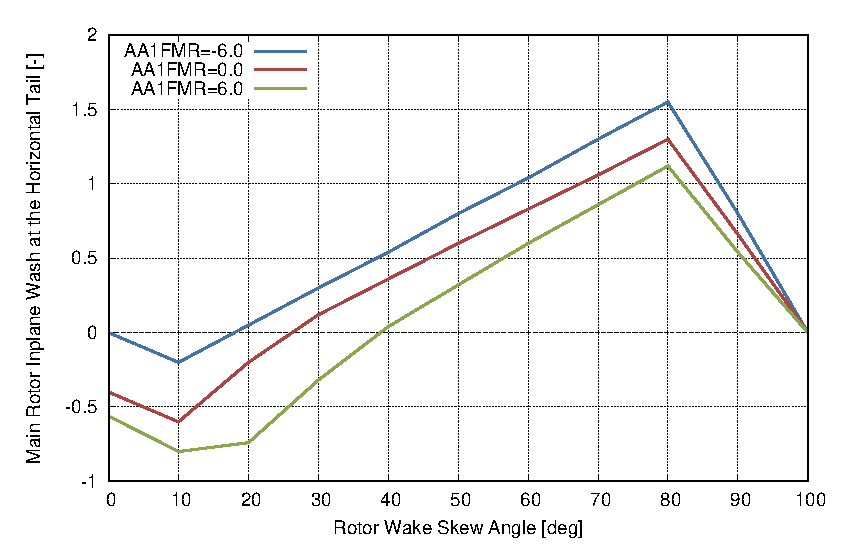
\includegraphics[width=140mm]{eps/uh60_stab_h_mr_inplane.eps}
  \caption{Main rotor inplane wash at the horizontal tail \cite{NASA-CR-166309}}
\end{figure}

%%%%%%%%%%%%%%%%%%%%%%%%%%%%%%%%%%%%%%%%%%%%%%%%%%%%%%%%%%%%%%%%%%%%%%%%%%%%%%%%

\clearpage
\subsection{Main Rotor Downwash at the Horizontal Tail}

\csvreader[
  no head,
  longtable=cccc,
  table head=
    \toprule
    $\chi$ & \multicolumn{3}{c}{EKZH1} \\
    {[deg]} & {AA1FMR=-6.0} & {AA1FMR=0.0} & {AA1FMR=6.0} \\ \midrule
    \endfirsthead
    $\chi$ & \multicolumn{3}{c}{EKZH1} \\
    {[deg]} & {AA1FMR=-6.0} & {AA1FMR=0.0} & {AA1FMR=6.0} \\ \midrule
    \endhead,
  before first line={},
  late after line=\\,
  late after last line=\\ \bottomrule \caption{Main rotor downwash at the horizontal tail \cite{NASA-CR-166309}},
  before reading={},
  after reading={}
]
{csv/uh60_stab_h_mr_downwash.csv}
{1=\colchi,2=\colii,3=\coliii,4=\coliv}
{\colchi & \colii & \coliii & \coliv}

\begin{figure}[h!]
  \centering
  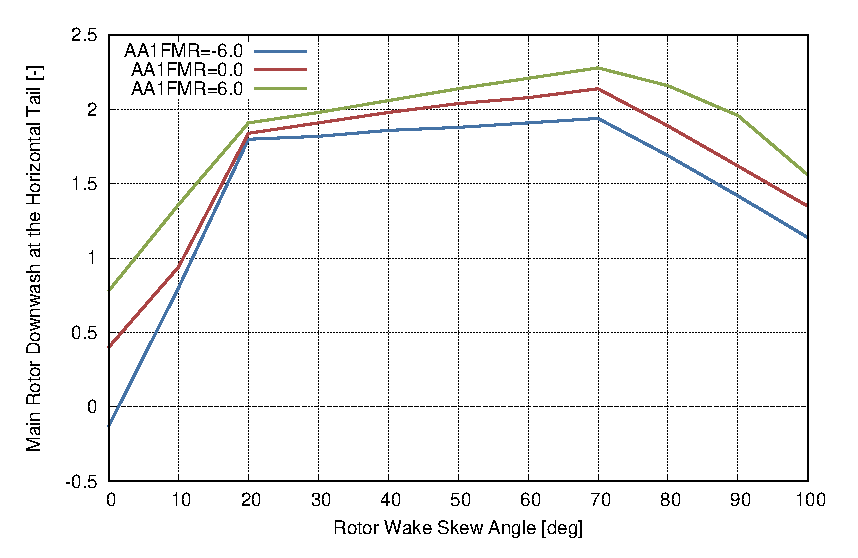
\includegraphics[width=140mm]{eps/uh60_stab_h_mr_downwash.eps}
  \caption{Main rotor downwash at the horizontal tail \cite{NASA-CR-166309}}
\end{figure}

%%%%%%%%%%%%%%%%%%%%%%%%%%%%%%%%%%%%%%%%%%%%%%%%%%%%%%%%%%%%%%%%%%%%%%%%%%%%%%%%

\clearpage
\subsection{Dynamic Pressure Loss at the Horizontal Tail}

\csvreader[
  no head,
  longtable=cc,
  table head=
    \toprule
    $\alpha$ & QH1QWF \\
    {[deg]} & {[-]} \\ \midrule
    \endfirsthead
    $\alpha$ & QH1QWF \\
    {[deg]} & {[-]} \\ \midrule
    \endhead,
  before first line={},
  late after line=\\,
  late after last line=\\ \bottomrule \caption{Dynamic pressure loss at the horizontal tail \cite{NASA-CR-166309}},
  before reading={},
  after reading={}
]
{csv/uh60_stab_h_press_loss.csv}
{1=\colaoa,2=\coldyn}
{\colaoa & \coldyn}

\begin{figure}[h!]
  \centering
  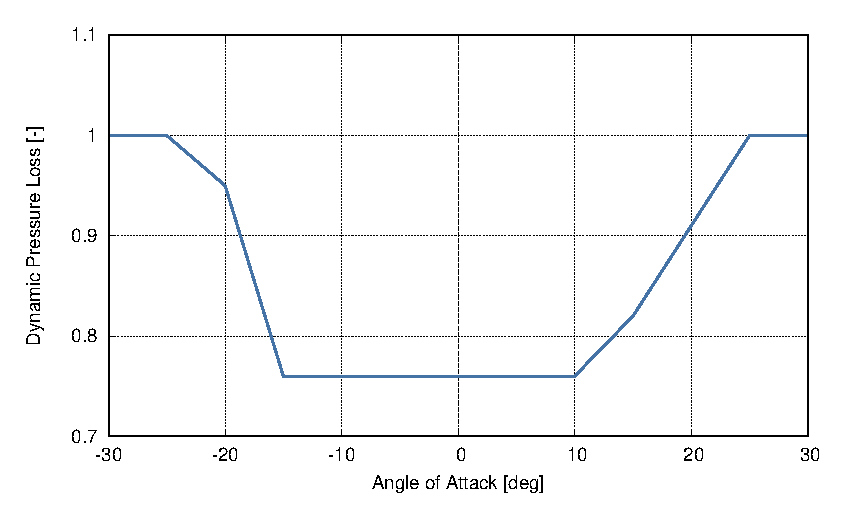
\includegraphics[width=140mm]{eps/uh60_stab_h_press_loss.eps}
  \caption{Dynamic pressure loss at the horizontal tail \cite{NASA-CR-166309}}
\end{figure}

%%%%%%%%%%%%%%%%%%%%%%%%%%%%%%%%%%%%%%%%%%%%%%%%%%%%%%%%%%%%%%%%%%%%%%%%%%%%%%%%

\clearpage
\subsection{Fuselage Downwash at the Horizontal Tail}

\csvreader[
  no head,
  longtable=cc,
  table head=
    \toprule
    $\alpha_f$ & $\epsilon_h$ \\
    {[deg]} & {[deg]} \\ \midrule
    \endfirsthead
    $\alpha_f$ & $\epsilon_h$ \\
    {[deg]} & {[deg]} \\ \midrule
    \endhead,
  before first line={},
  late after line=\\,
  late after last line=\\ \bottomrule \caption{Fuselage downwash at the horizontal tail \cite{NASA-CR-166309}},
  before reading={},
  after reading={}
]
{csv/uh60_stab_h_f_downwash.csv}
{1=\colaoa,2=\coleps}
{\colaoa & \coleps}

\begin{figure}[p!]
  \centering
  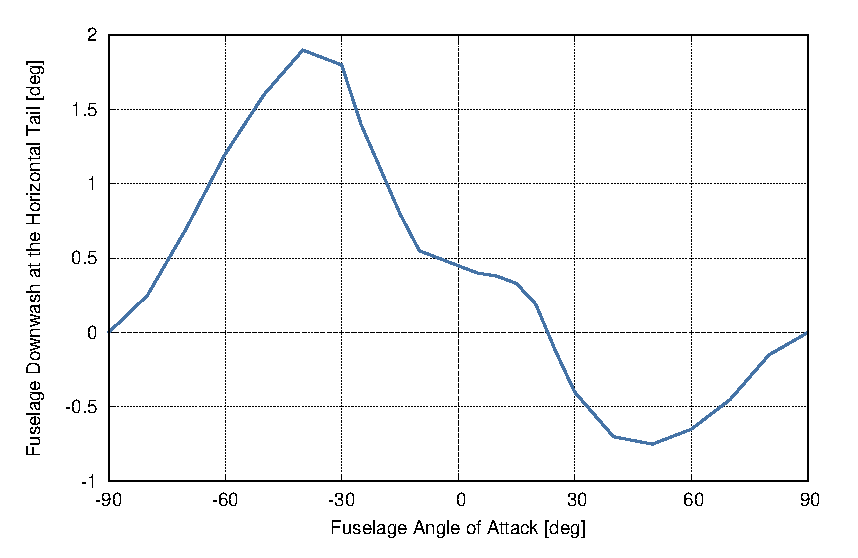
\includegraphics[width=140mm]{eps/uh60_stab_h_f_downwash.eps}
  \caption{Fuselage downwash at the horizontal tail \cite{NASA-CR-166309}}
\end{figure}

%%%%%%%%%%%%%%%%%%%%%%%%%%%%%%%%%%%%%%%%%%%%%%%%%%%%%%%%%%%%%%%%%%%%%%%%%%%%%%%%

\clearpage
\subsection{Horizontal Tail Aerodynamic Coefficients}

\csvreader[
  no head,
  longtable=ccc,
  table head=
    \toprule
    $\alpha$ & $C_{X,h}$ & $C_{Z,h}$ \\
    {[deg]} & {[-]} & {[-]} \\ \midrule
    \endfirsthead
    $\alpha$ & $C_{X,h}$ & $C_{Z,h}$ \\
    {[deg]} & {[-]} & {[-]} \\ \midrule
    \endhead,
  before first line={},
  late after line=\\,
  late after last line=\\ \bottomrule \caption{Horizontal tail aerodynamic coefficients \cite{NASA-CR-166309}},
  before reading={},
  after reading={}
]
{csv/uh60_aero_stab_h.csv}
{1=\colaoa,2=\colhcx,3=\colhcz}
{\colaoa & \colhcx & \colhcz}

\begin{figure}
  \centering
  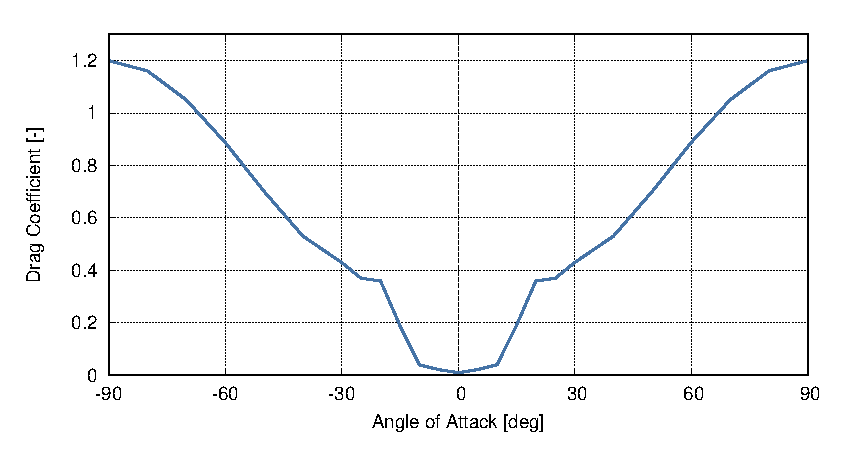
\includegraphics[width=140mm]{eps/uh60_stab_h_cx.eps}
  \caption{Horizontal tail drag coefficient due to angle of attack \cite{NASA-CR-166309}}
\end{figure}

\begin{figure}
  \centering
  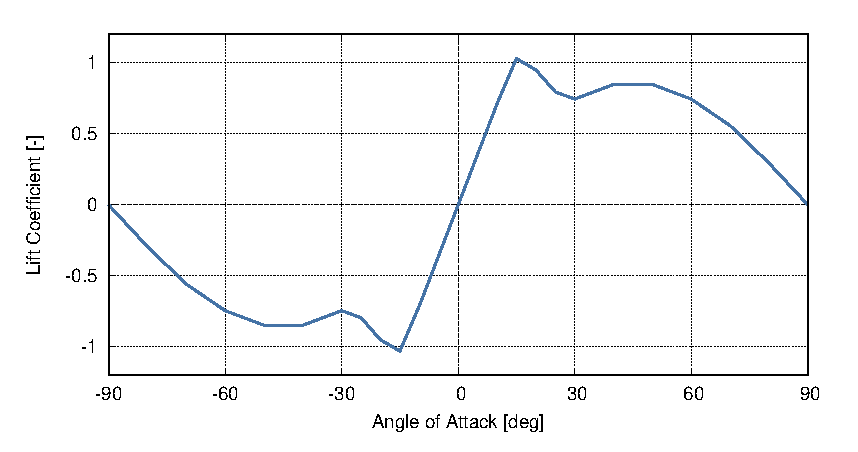
\includegraphics[width=140mm]{eps/uh60_stab_h_cz.eps}
  \caption{Horizontal tail lift coefficient due to angle of attack \cite{NASA-CR-166309}}
\end{figure}

%%%%%%%%%%%%%%%%%%%%%%%%%%%%%%%%%%%%%%%%%%%%%%%%%%%%%%%%%%%%%%%%%%%%%%%%%%%%%%%%

\clearpage
\subsection{Dynamic Pressure Loss at the Vertical Tail}

\csvreader[
  no head,
  longtable=cc,
  table head=
    \toprule
    $\beta$ & QP3QWF \\
    {[deg]} & {[-]} \\ \midrule
    \endfirsthead
    $\beta$ & QP3QWF \\
    {[deg]} & {[-]} \\ \midrule
    \endhead,
  before first line={},
  late after line=\\,
  late after last line=\\ \bottomrule \caption{Dynamic pressure loss at the vertical tail \cite{NASA-CR-166309}},
  before reading={},
  after reading={}
]
{csv/uh60_stab_v_press_loss.csv}
{1=\colbeta,2=\coldyn}
{\colbeta & \coldyn}

\begin{figure}[h!]
  \centering
  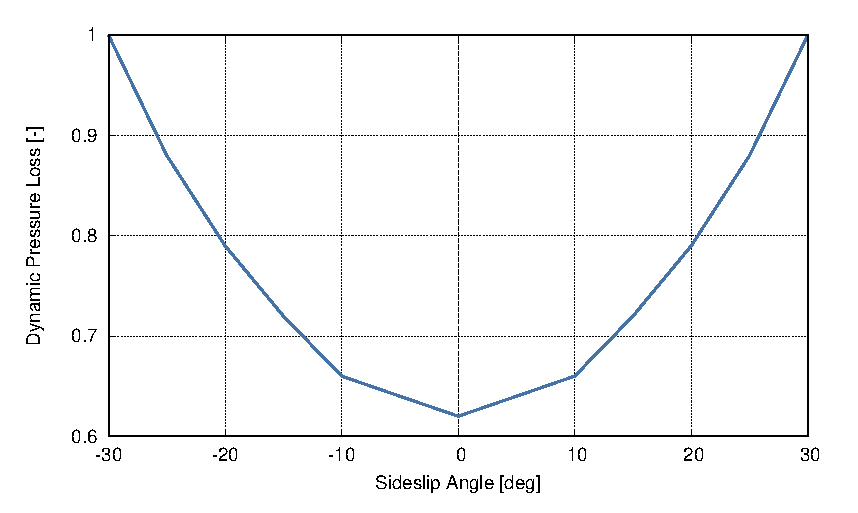
\includegraphics[width=140mm]{eps/uh60_stab_v_press_loss.eps}
  \caption{Dynamic pressure loss at the vertical tail \cite{NASA-CR-166309}}
\end{figure}

%%%%%%%%%%%%%%%%%%%%%%%%%%%%%%%%%%%%%%%%%%%%%%%%%%%%%%%%%%%%%%%%%%%%%%%%%%%%%%%%

\clearpage
\subsection{Fuselage Sidewash at the Vertical Tail}

\csvreader[
  no head,
  longtable=cc,
  table head=
    \toprule
    $\beta_f$ & $\epsilon_v$ \\
    {[deg]} & {[deg]} \\ \midrule
    \endfirsthead
    $\beta_f$ & $\epsilon_v$ \\
    {[deg]} & {[deg]} \\ \midrule
    \endhead,
  before first line={},
  late after line=\\,
  late after last line=\\ \bottomrule \caption{Fuselage sidewash at the vertical tail \cite{NASA-CR-166309}},
  before reading={},
  after reading={}
]
{csv/uh60_stab_v_f_sidewash.csv}
{1=\colbeta,2=\coleps}
{\colbeta & \coleps}

\begin{figure}[p!]
  \centering
  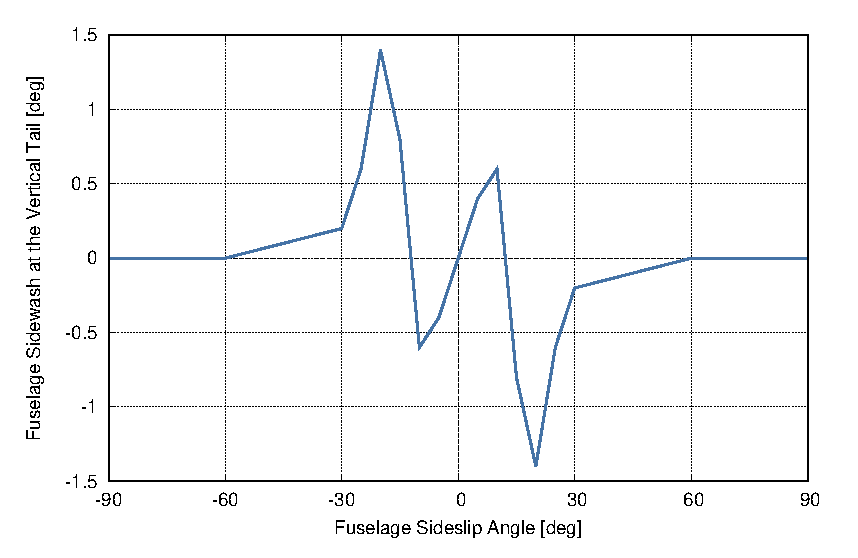
\includegraphics[width=140mm]{eps/uh60_stab_v_f_sidewash.eps}
  \caption{Fuselage sidewash at the vertical tail \cite{NASA-CR-166309}}
\end{figure}

%%%%%%%%%%%%%%%%%%%%%%%%%%%%%%%%%%%%%%%%%%%%%%%%%%%%%%%%%%%%%%%%%%%%%%%%%%%%%%%%

\clearpage
\subsection{Vertical Tail Aerodynamic Coefficients}

\csvreader[
  no head,
  longtable=ccc,
  table head=
    \toprule
    $\beta$ & $C_{X,v}$ & $C_{Y,v}$ \\
    {[deg]} & {[-]} & {[-]} \\ \midrule
    \endfirsthead
    $\beta$ & $C_{X,v}$ & $C_{Y,v}$ \\
    {[deg]} & {[-]} & {[-]} \\ \midrule
    \endhead,
  before first line={},
  late after line=\\,
  late after last line=\\ \bottomrule \caption{Vertical tail aerodynamic coefficients \cite{NASA-CR-166309}},
  before reading={},
  after reading={}
]
{csv/uh60_aero_stab_v.csv}
{1=\colbeta,2=\colvcx,3=\colvcy}
{\colbeta & \colvcx & \colvcy}

\begin{figure}
  \centering
  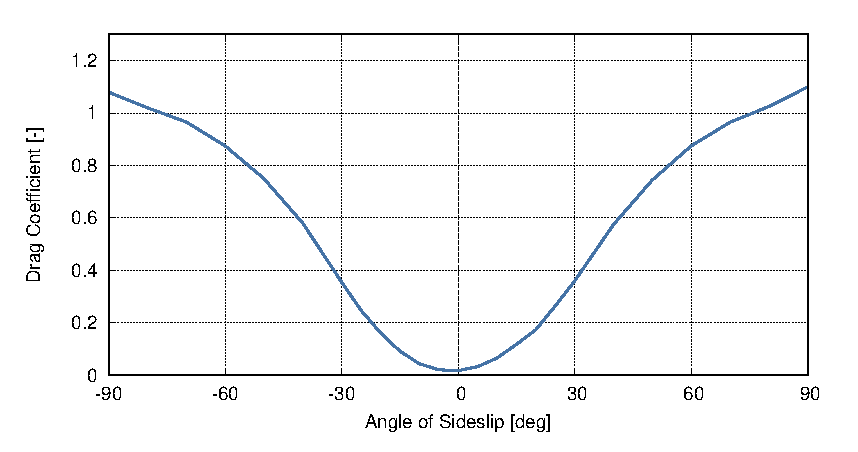
\includegraphics[width=140mm]{eps/uh60_stab_v_cx.eps}
  \caption{Vertical tail drag coefficient due to sideslip \cite{NASA-CR-166309}}
\end{figure}

\begin{figure}
  \centering
  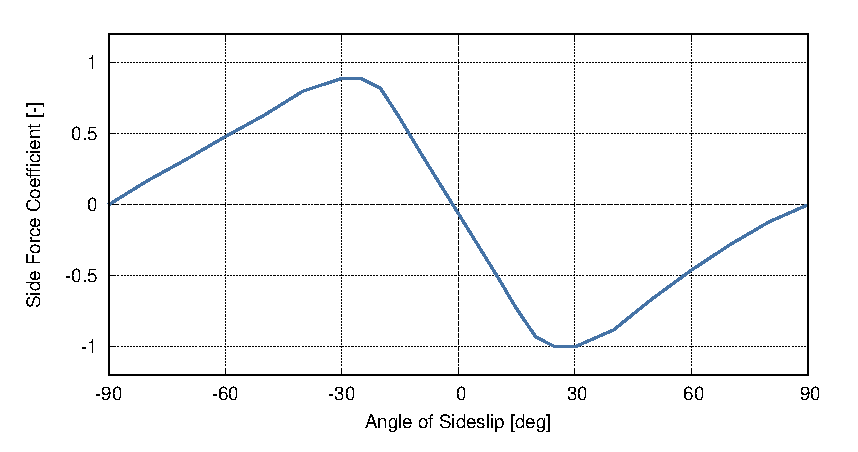
\includegraphics[width=140mm]{eps/uh60_stab_v_cy.eps}
  \caption{Vertical tail side force coefficient due to sideslip \cite{NASA-CR-166309}}
\end{figure}
